SAMPLING

The sampling of the data is performed using the ADAU1761 chip of the zedboard.
It is a coder / decoder that samples the voltage level coming from the line in,
and can also output it on the line out and do all sorts of transformation.
The process of sampling has been facilitated by the use of the interface 
developed by Mike Field \cite{github/audio}.
It provides 24 bit samples in two's complement at 48kHz.
\begin{figure}
    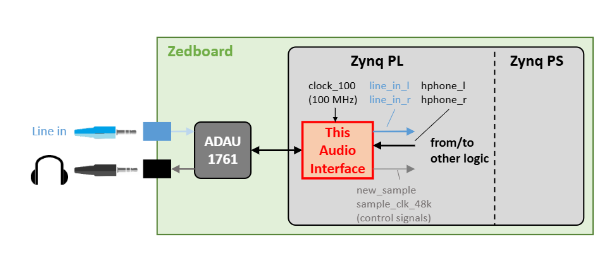
\includegraphics[width=0.8\textwidth]{figures/Audio_interface.png}
    \caption{This is a figure}
\end{figure}
\begin{figure}
    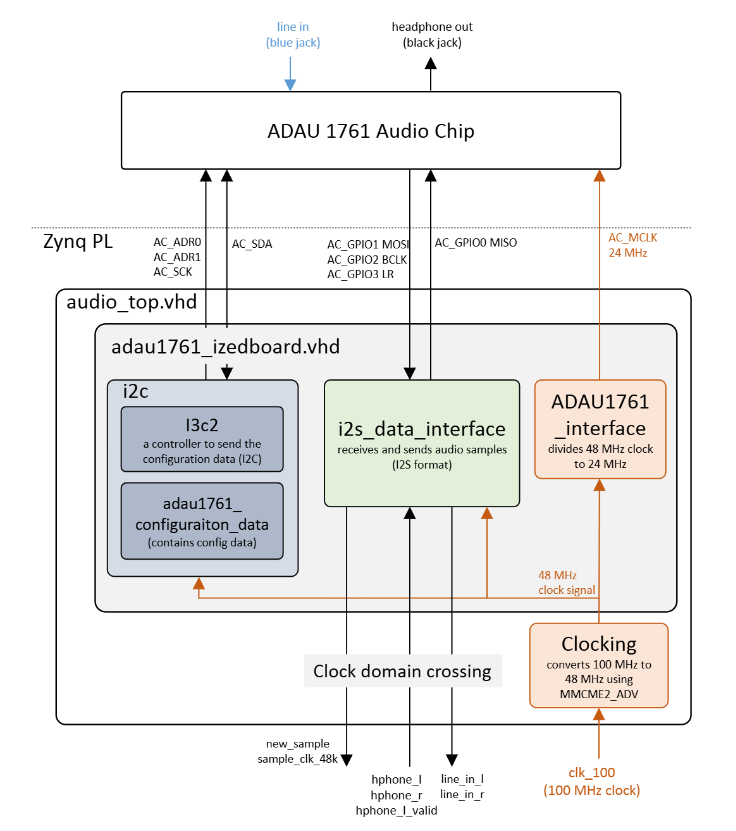
\includegraphics[width=0.8\textwidth]{figures/audio_interface_BD.png}
\end{figure}

DOWNSAMPLING

